\section{Introducción}
Este Trabajo de Fin de Grado se enfoca en el desarrollo de un juego para asistentes conversacionales, dirigido a adultos mayores en residencias o centros de día, que pueden ser propensos a aislarse a pesar de estar rodeadas de otras personas. Reconociendo los desafíos que enfrenta este grupo demográfico en la era digital, el proyecto busca integrar una de las tecnologías más punteras de manera accesible y lúdica. Por tanto, el objetivo es no solo fomentar la conexión social en estos espacios, sino también promover la estimulación cognitiva y el bienestar emocional de las personas mayores.

Dado que las personas mayores están menos familiarizadas con el uso de herramientas digitales en su vida cotidiana puede parecer difícil que se sientan atraídas por juegos que se basan en la tecnología, sin embargo si las personas usuarias en un primer momento comprueban que no solo pueden acceder a este entretenimiento si no que, además se incentivan sus relaciones personales, conocen nuevas amistades y se abre un mundo nuevo de ocio y desarrollo intelectual, se podrá ver cómo conduce a un envejecimiento más saludable.

La idea detrás de este TFG podría resumirse con la siguiente cita: \enquote{Las actividades físicas, cognitivas y emocionales en edades avanzadas son cruciales para estimular la actividad cerebral y contribuir al mantenimiento de la calidad de vida. Además de los beneficios físicos y cerebrales, los juegos estimulan la interacción social y contribuyen a la socialización y al mantenimiento de la salud emocional y afectiva} \parencite{intro3}.


\subsection{Motivación y contexto}

Este TFG se integra dentro del proyecto de investigación \enquote{Evaluación del uso de robots sociales y sistemas conversacionales en residencias y centros de día para promover el envejecimiento saludable} de la Universidad de Granada, con  la profesora Nuria Medina Medina como investigadora principal del mismo, y directora de este Trabajo de Fin de Grado.

Este proyecto, con código C-ING-179-UGR23, \enquote{propone el uso y evaluación de Agentes Sociales Interactivos (SIA - Social Interactive Agent) (en particular de Robots Sociales apoyados por Asistentes Conversacionales) que promuevan el envejecimiento saludable y las interacciones sociales de los mayores en la residencia o centro de día, ya que estas interacciones son muy importantes para el mejoramiento de la salud y estado anímico de los mayores. Para maximizar su efectividad, la propuesta integrará experiencias lúdicas y técnicas de interacción multimodal}. 

Dicho proyecto destaca por su metodología pionera en relación con el estado del arte ya que se focaliza en la utilización de los robots sociales para fomentar el envejecimiento saludable y mejorar la comunicación y los problemas de interacción social en las residencias. El proyecto también se centra en el diseño de experiencias lúdicas integradas en entornos sociales para favorecer los problemas de motivación y adopción de la tecnología.

Que el uso de la tecnología puede ser un apoyo importante para lograr una mayor calidad de vida en los adultos mayores que viven en residencias o asisten a centros de día es una de las premisas en las que se apoya la investigación. \enquote{Consecuentemente, este proyecto propone el uso y evaluación de Agentes Sociales Interactivos (SIA - Social Interactive Agent) (en particular de Robots Sociales apoyados por Asistentes Conversacionales) que promuevan el envejecimiento saludable y las interacciones sociales de los mayores en la residencia o centro de día, ya que estas interacciones son muy importantes para el mejoramiento de la salud y estado anímico de los mayores. Para maximizar su efectividad, la propuesta integrará experiencias lúdicas y técnicas de interacción multimodal}.

Según se menciona en el artículo \textit{La soledad y el aislamiento social en las personas mayores} \parencite{ArruebarrenaCabaco2020}, \enquote{El aislamiento social se define como una ausencia objetiva de relaciones/contactos sociales y la soledad como la experiencia subjetiva aversiva que se siente al valorar esas relaciones/contactos sociales como
insuficiente en cantidad y/o calidad}

En los últimos tiempos, el tema de la soledad en las personas mayores ha ganado atención en los medios de comunicación, describiéndose como una \enquote{epidemia} en aumento. Aunque no hay evidencia sólida que respalde la idea de una nueva epidemia, las dificultades metodológicas y la falta de consenso en la medición de la soledad limitan la capacidad de confirmar si las personas mayores se sienten más solas que antes.

A pesar de estas limitaciones, estudios indican tasas de soledad entre las personas mayores en España, oscilando entre el 14\% y el 24\%, e incluso alcanzando el 40\% en algunos casos. Uno de los factores que contribuyen a esta percepción es el aumento en el número de personas mayores viviendo solas. Se proyecta que para 2050, aproximadamente un tercio de la población tendrá más de 65 años, lo que por lógica implica un aumento en el número de personas mayores que viven solas.

\begin{figure}[ht]
    \centering
    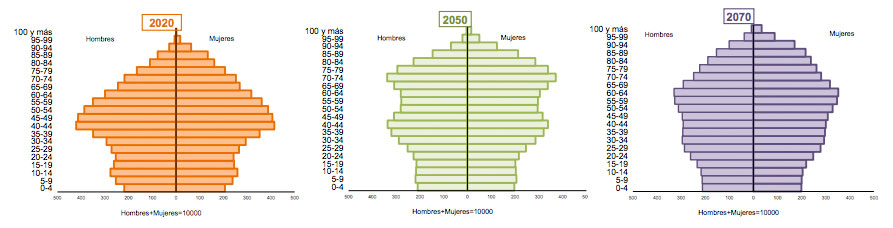
\includegraphics[width=0.98\textwidth]{imgs/piramide-poblacion.jpg}
    \caption{Pirámides de población de España en futuros años (\href{https://www.geriatricarea.com/2020/09/25/uno-de-cada-tres-espanoles-tendra-65-o-mas-anos-en-el-2050/}{geriatricarea.com})}
    \label{fig:piramide-poblacion}
\end{figure}

El aumento de la esperanza de vida de la población adulta en nuestro país ha supuesto que las personas mayores, muchas de ellas que viven solas y poseen nivel económico y cultural medio, supongan un sector amplio de la población que requiere de nuevas formas de ocio y de relacionarse socialmente. Muchas de estas personas viven solas y el sedentarismo y la falta de interacción social les produce que su desarrollo cognitivo se vea mermado.

También la frecuente automarginación de este grupo demográfico para el uso de herramientas digitales como juegos o aplicaciones, el fenómeno conocido de forma general como brecha digital, contribuye a un mayor aislamiento social. \enquote{Muchos adultos mayores tienen acceso a dispositivos móviles, pero no pueden aprovecharlos completamente debido a la falta de conocimiento o el miedo a salir de su zona de confort. Esto resulta en barreras emocionales, dificultades para adquirir nuevas habilidades tecnológicas} \parencite{intro1}. 

A pesar de lo mencionado en el párrafo anterior, el segmento de edad mayor de 60 años no es ajeno a la realidad de que las formas de socialización del siglo XXI están vinculadas a los avances tecnológicos y a las nuevas experiencias lúdicas. Como se señala en \textit{Las competencias digitales en personas mayores: de amenaza a oportunidad}: \enquote{el potencial que para las personas mayores ofrece el uso habitual de las TIC es enorme, con una larga lista de oportunidades existentes para el beneficio de este colectivo que deben ser aprovechadas} \parencite{intro4}.

Un juego digital que suponga entretenimiento para las personas mayores, al mismo tiempo que una mejora de memoria y ampliación de lenguaje y percepción puede significar un estimulante cambio en su día a día. 

\subsubsection{Impacto social y tecnológico de la pandemia de COVID-19}

Durante la pandemia por el COVID-19 millones de personas en el mundo tuvieron que pasar en pocos días de trabajo presencial al online y en sus relaciones personales debieron adaptar sus costumbres al nuevo escenario virtual.

De esta manera, personas acostumbradas a comunicarse solo por llamadas telefónicas, y muy poco mediante telefonía móvil, se volvieron usuarias de videollamadas diarias ante la necesidad de mantenerse conectados con familiares y amigos, combinada con las restricciones de movimiento.

Este cambio tuvo un impacto profundo en la vida diaria de las personas mayores. Por un lado, les brindó una forma vital de mantenerse conectados con sus seres queridos, incluso cuando no podían reunirse físicamente debido a las medidas de distanciamiento social. Esto ayudó a reducir un poco el riesgo de aislamiento social y proporcionó un medio para el apoyo emocional y la interacción social, lo cual es esencial para su bienestar mental y emocional.

Sin embargo, la transición a las tecnologías digitales también presentó desafíos, especialmente para aquellos menos familiarizados con ellas. Algunos enfrentaron dificultades técnicas al principio, como la configuración de aplicaciones o la resolución de problemas de conexión. Además, la dependencia excesiva de la tecnología para la comunicación también puede aumentar la brecha digital entre aquellos que tienen acceso y conocimientos tecnológicos y aquellos que no los tienen, lo que potencialmente podría aumentar el riesgo de exclusión social para algunos adultos mayores.

A pesar de estos desafíos, la pandemia actuó como un catalizador para la adopción de tecnología entre las personas mayores, lo que les permitió permanecer conectados y participar en la sociedad de manera más activa, incluso en tiempos de crisis. Como resultado, muchas personas mayores han incorporado el uso de tecnologías digitales en su vida diaria incluso después de que levantaran las restricciones de la pandemia, lo que les brinda nuevas oportunidades de participación social y acceso a recursos y servicios en línea \parencite{intro2}.

Según datos del Instituto Nacional de Estadística (INE), la población que usa Internet (en los últimos meses el uso de las tecnologías de información y comunicación (TIC) en los hogares ha crecido en los últimos años, si bien sigue existiendo una brecha entre los usuarios y no usuarios (brecha digital) que se puede atribuir a una serie de factores: la falta de infraestructura (en particular en las zonas rurales), la falta de conocimientos de informática y habilidades necesarias para participar en la sociedad de la información, o la falta de interés en lo que la sociedad de la información puede ofrecer).

Al aumentar la edad desciende el uso de Internet, siendo el porcentaje más bajo el que corresponde al grupo de edad de 65 a 74 años (un 79,7\% para los hombres y un 80,5\% para las mujeres) \parencite{intro5}.

\begin{figure}[H]
	\centering
	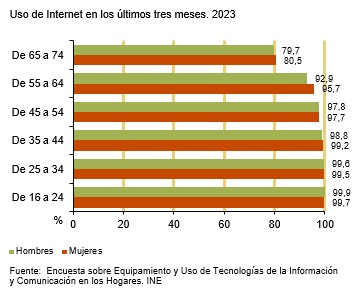
\includegraphics{imgs/INE-grafica1.jpeg}
	\caption{Población por grupos de edad que han usado Internet en los últimos tres meses (INE, 2018-23)}
	\label{fig:grafica1-INE}
\end{figure}

\begin{figure}[H]
	\centering
	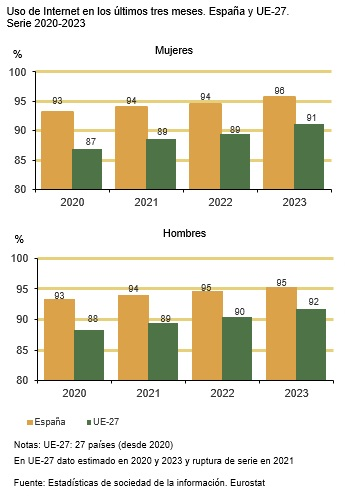
\includegraphics{imgs/INE-grafica2.jpeg}
	\caption{Población de entre 16 y 74 años que ha usado Internet en los últimos tres meses en la UE (INE, 2020-23)}
	\label{fig:grafica2-INE}
\end{figure}

Según una encuesta realizada por Canal Sénior, plataforma online de entretenimiento y aprendizaje para personas mayores de 55 años, entre sus usuarios, en el capítulo de juegos y aplicaciones de entretenimiento: \enquote{la mayoría de los encuestados prefieren los juegos que permiten el entrenamiento mental, como aplicaciones del tipo Trivial, Apalabrados, Scrabble, Wordle, etc. Esto es muy relevante en personas sénior, pues está probado que los juegos que retan a la mente y nos hacen pensar pueden retrasar el envejecimiento cognitivo durante más tiempo}.

Todo hace indicar que cada vez hay una relación más estrecha entre mayores y ocio digital. \enquote{Es también relevante ver cómo algunos de sus gustos y preferencias son diferentes a los de otros grupos de edad, como por ejemplo su preferencia por la lectura al consumo de series y películas o de contenidos en las redes sociales. Por último, conviene destacar que el uso de las tecnologías digitales como parte de nuestro ocio pueden ayudarnos a tener un envejecimiento activo, sano y con participación elevada en la sociedad.} \parencite{intro6}.

\subsection{Objetivos}
El presente trabajo tiene como objetivo desarrollar un juego digital, que contribuya al creciente conjunto de soluciones innovadoras para combatir el aislamiento social en los adultos mayores alojados en residencias o centros de día.

Este juego no solo buscará proporcionar entretenimiento y diversión, sino que también se centrará en promover la participación, el compromiso cognitivo y emocional, y en general, mejorar la calidad de vida de las personas mayores. 

Para lograr este objetivo principal, se puede descomponer en varios subobjetivos, recogidos en la siguiente tabla:

\begin{table}[ht]
  \centering
  \begin{tabular}{| c | p{9.6cm} |}
    \hline
    \rowcolor{lightgray}
    \textbf{Subobjetivo} & \textbf{Descripción} \\
    \hline
    1. Revisión de la literatura & 
        1.1. Identificar las investigaciones clave sobre el impacto del aislamiento social en personas mayores \newline
        \vspace{0.2cm}
        1.2. Analizar la diversidad de intervenciones digitales dirigidas a este grupo demográfico \vspace{0.2cm} \\
    \hline
    2. Diseño del juego &
        2.1. Investigar las mejores prácticas en el diseño de juegos digitales accesibles para personas mayores \newline
        \vspace{0.2cm}
        2.2. Considerar las adaptaciones necesarias para abordar posibles limitaciones físicas y cognitivas
        \vspace{0.2cm} \\
    \hline
    3. Desarrollo técnico & 
        3.1. Seleccionar la plataforma y tecnologías más apropiadas para el desarrollo del juego \newline
        \vspace{0.2cm}
        3.2. Asegurar la compatibilidad con dispositivos comunes utilizados por personas mayores \newline
        \vspace{0.2cm}
        3.3. Integrar funcionalidades de accesibilidad, como ajustes de tamaño de fuente y navegación simplificada \vspace{0.2cm} \\
    \hline
    4. Contribución al conocimiento & 
    4.1. Contribuir al creciente cuerpo de conocimientos sobre cómo la tecnología puede mejorar la calidad de vida de los adultos mayores, particularmente en el contexto de residencias y centros de día. 
    \vspace{0.2cm} \\
    \hline
    5. Participación comunitaria & 
        5.1. Colaborar con comunidades de personas mayores para obtener retroalimentación. \newline
        \vspace{0.2cm}
        5.2. Organizar pruebas piloto y grupos de enfoque para evaluar la experiencia del usuario. \vspace{0.2cm} \\
    \hline
    \end{tabular}
  \caption{Subobjetivos del trabajo.}
  \label{tab:subobjetivos}
\end{table}